\documentclass[a4paper,10pt]{article}
\usepackage[utf8]{inputenc}

% \usepackage[T1]{fontenc}
% \usepackage{tgbonum}

\usepackage{tikz}
\usetikzlibrary{calc,fadings,shadings}

\usepackage{array}
\usepackage{tabularx}

\usepackage[noheadfoot, nomarginpar, landscape, margin=.5in, verbose]{geometry}

\usepackage{hyperref}

\usepackage{xcolor}

\usepackage{booktabs}

\usepackage{fontawesome}

\usepackage[backend=biber,maxcitenames=1,doi=false,isbn=false,url=false]{biblatex}
\addbibresource{thesis.bib}

% Done:
% - enlever le "present" dans les teachings, tu n'enseignes plus
% - mettre ton nom en un peu plus visible (\Large > \LARGE)
% - mettre des exemples de rpg
% - dans les publications, mettre le "ed" en décalé par rapport aux bullets points comme s'il avait une tabulation (enough?)
% - dans les teachings décaler plus les bullets points blanches vers la droite (enough?)
% - les boutons de chargement dans les computing skills ne rendent pas. On dirait des bullets points classiques.
% - mettre des genres de lecture pas des auteurs
% - je préfèrerais avoir des chemins rouges qui mènent à chaque rubrique
%
% Unsure:
% 
%
% Pending:
% - l'adresse mail irit va-t-elle être pertinente longtemps ?
% 
% - décomposer l'anglais en writing, listening, hearing et du coup changer le nom de ta section en juste "languages"
% 
% - t'as mis 2x rpg dans les loisirs, ça fait nerd
% 
% - mettre les mentions des diplomes si tu le souhaites

\title{CV - Kevin Godin-Dubois}
\makeatletter
\hypersetup{
 pdfinfo={
  Author={Kevin Godin-Dubois},
  Title={\@title}
 }
}
\makeatother

\begin{document}
\def\ifdrawguidelines{\iffalse}

\newlength{\innersep}
\setlength{\innersep}{5pt}
\tikzset{
 sect/.style={
%   draw,
  inner sep=\innersep
 }
}
\newcommand{\nsect}[5][]{
 \setlength{\tabcolsep}{0pt}
 \node [sect, #1] (#2) {
  \begin{sect}{#3}{#5}
    #4
  \end{sect}
 };
}
\newenvironment{sect}[2]
               {\begin{tabular}{m{\dimexpr#2-2\innersep\relax}}\multicolumn{1}{c}{\large\textbf{#1}}\\}
               {\end{tabular}}

\newcommand{\itm}[2]{\\\textbf{#1} - #2}

\pgfmathsetlengthmacro\D{.2*\textwidth}
\pgfmathsetlengthmacro{\R}{.5*\D}
\thispagestyle{empty}

\setlength\parindent{24pt}

\def\di{$\bullet$\ }
\def\dii{\hspace{1.5em} $\circ$\ }

\tikzfading[name=fade out,inner color=transparent!0,outer color=transparent!100]
\def\sbcolor{red}
\newcommand{\skillbar}[1]{
 \begin{tikzpicture}
  \def\sbx{0}
  \def\sby{0}
  \def\sbwA{.66\textwidth}
  \pgfmathsetmacro{\sbwB}{#1 / 100 * .66\textwidth}
  \def\sbh{.1cm}
  \def\sbr{1.5pt}
  
  \draw [\sbcolor, rounded corners=\sbr] (\sbx,\sby) rectangle (\sbwA,\sbh);
  \path [clip, rounded corners=\sbr] (\sbx,\sby) rectangle (\sbwB pt,\sbh);
  \fill [\sbcolor] (\sbx,\sby) rectangle (\sbwB pt,\sbh); 
  \fill [\sbcolor!50!black,path fading=fade out] (-\sbwB pt,\sby+\sbh) rectangle (\sbwB pt,-\sbh);
  \fill [\sbcolor!20!white,path fading=fade out] (0,\sby+2*\sbh) rectangle (2*\sbwB pt,0);
 \end{tikzpicture}
}

\newcommand{\skilldisk}[1]{
 \hspace{.5em}
 \begin{tikzpicture}
  \def\R{.15cm}
  \pgfmathsetmacro\A{90-3.6*#1}
  \def\bgcolor{gray!40}
  \def\fgcolor{\sbcolor!50}
  
  \fill [white] (0,0) circle (\R);
  \draw [\bgcolor] (\A:\R) arc (\A:-270:\R);
  \draw [\fgcolor] (\A:\R) -- (0,0) -- (90:\R) arc (90:\A:\R) -- cycle;
  
  \shade[ball color = \bgcolor, opacity = 0.4] (0,0) circle (\R);
  \shade[ball color = \fgcolor, opacity = 0.8] (0,\R) arc (90:\A:\R) -- (0,0) -- cycle;
 \end{tikzpicture}
}

\def\skilllevel{\skilldisk}

\begin{tikzpicture}[remember picture, overlay]
 \node (page) at (current page.center) [minimum width=\textwidth, minimum height=\textheight] {};
 
 \ifdrawguidelines
  \foreach \a in {center, north, east, west, south, north east, north west, south west, south east} { \node [draw] at (\a) {\a}; }
  \tikzset{guideline/.style={dotted,gray,thick}}
  \draw [guideline] (north) -- (south);
  \draw [guideline] (west) -- (east);
  \draw [guideline] (east) -- (north) -- (west) -- (south) -- cycle;
  \draw [guideline] (north east) -- (north west) -- (south west) -- (south east);
 \fi
 
 
 \def\angle{0}
 \def\aPhase{82.5}
 \foreach \n/\a in {\aPI/141.5, \aEd/-86.5, \aPE/-57.5, \aPC/-87.5, \aCS/-69.5, \aMi/-32} {
  \pgfmathsetmacro{\angle}{\angle+\a} \xdef\angle{\angle} \expandafter\xdef\n{\angle}
 }

 \node [rotate=\aPI-\aPhase] (C) at (page.center) {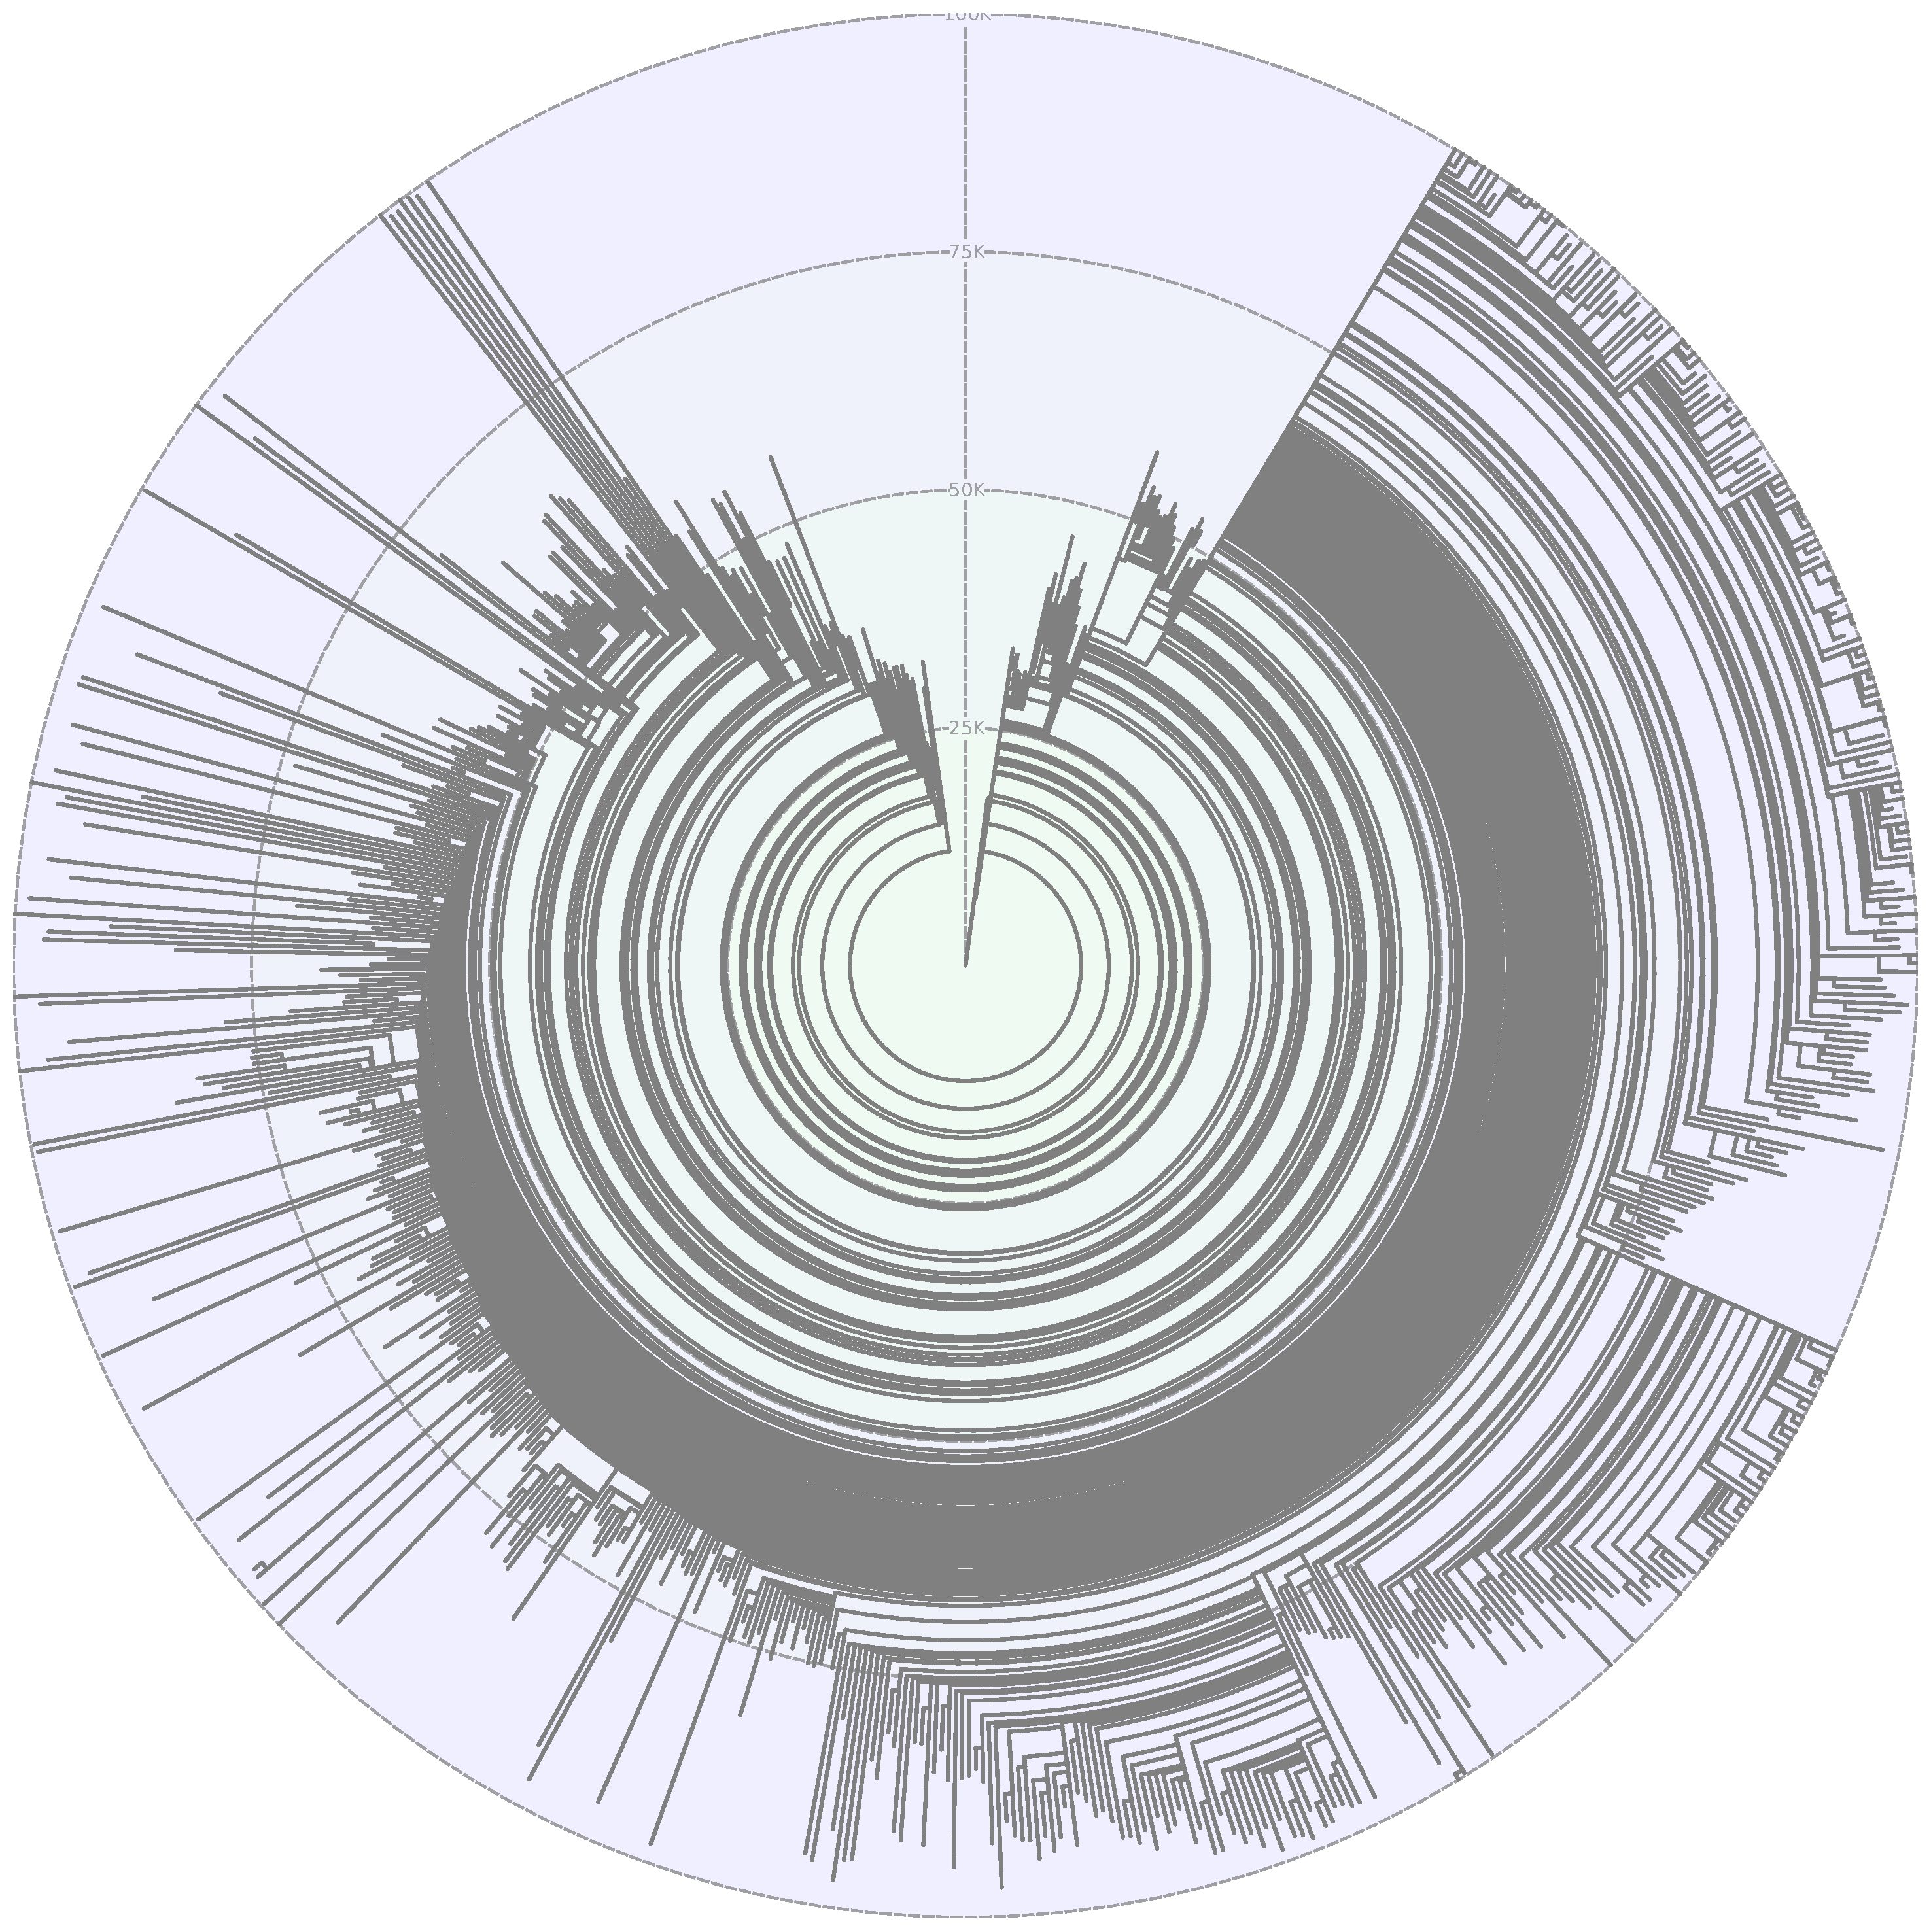
\includegraphics[width=\D]{annexes/phylogenetics_monochrome}};

 \def\v{.2cm}
 \nsect[anchor=north west,at={(page.north west)}]{PI}{\LARGE Kevin Godin-Dubois}{
  \addlinespace[\v]
  \multicolumn{1}{c}{\large \emph{A-Life Researcher on the Emergence of Cognition}} \\
  \addlinespace[\v]
  \begin{tabular}{c@{ }m{.158\textwidth}c@{ }m{.11\textwidth}}
   \faHome & University of Toulouse & \faPhone & +33 5 67 06 93 91 \\
           & IRIT - CNRS UMR 5505   & \faMobile & +33 6 18 72 09 06 \\
           & \multicolumn{3}{l}{2 rue du Doyen Gabriel Marty} \\
           & 31042 Toulouse, France & \\
   \addlinespace[.1cm]
   \faEnvelopeO & \href{mailto:kevin.dubois@irit.fr}{kevin.dubois@irit.fr} &
       \faVimeo & \href{https://vimeo.com/godinduboisalife}{godinduboisalife} \\
      \faGithub & \href{https://github.com/kgd-al}{kgd-al@github.com} &
     \faRefresh & \href{https://github.com/kgd-al/CV/raw/master/cv.pdf}{Up-to date version} \\
  \end{tabular}
 }{.32\textwidth}
 
 \nsect[anchor=north east,at={(page.35)}]{Ed}{Education}{
  \begin{minipage}{.275\textwidth}
   \begin{tabular}{m{\textwidth}}
    \itm{2016-Present}{Capitole University, Toulouse} \\
    \emph{PhD thesis, ``Environment driven speciation''} \\
    { \small Investigated how complexification of artificial creatures could be further enhanced by moving the control apparatus around the abiotic component of an ecosystem } \\
    \\
   \end{tabular}
  \end{minipage}
  \hfill
  \begin{minipage}{.275\textwidth}
   \begin{tabular}{m{\textwidth}}
    \itm{2014-2016}{Paul Sabatier University, Toulouse} \\
    \emph{Master's degree in Computer Science} \\
    {\small Artificial intelligence: mathematical and symbolic models, training methods} \\
  
    \itm{2011-2014}{Paul Sabatier University, Toulouse} \\
    \emph{Bachelor's degree in Computer Science}
   \end{tabular}
  \end{minipage}
 }{.6\textwidth}
 
 \nsect[anchor=north east, at={(page.19)}]{PE}{Professional Experience}{
  \itm{2016-2019}{Teachings} \\
  \di 2017 \& 2018, Capitole University, Toulouse \\
  \dii L2 Excel and Visual Basic for Applications \\
  \dii L2 Algorithms and Visual Basic \\
  \dii L3 Modeling in Database \\
  \di 2016 \& 2017, Paul Sabatier University, Toulouse \\
  \dii L2 project monitoring on C programming \\
  
  \itm{2016}{Internship IRIT, France} \\
  {\small \textsc{Toulouse Research Institute on Computer Science}} \\
  \emph{``Rule-based artificial embryogenesis in a complex 3D environment''} \\
  {\small Deployed rule-based genomes on the MecaCell platform to study artificial plant growth and cell specialization.} \\
  \itm{2015}{Internship IRIT, France} \\
  \emph{``Comparison of different evolutionary approaches, an application to the GECCO 2015 challenge''} \\
  {\small Performed a performance comparison (accuracy, efficiency) between Artificial Neural and Genetic Regulatory Networks on the 2015 GECCO temperature prediction challenge data.} \\
 }{.35\textwidth}
 
 \nsect[anchor=south west, at={(page.south west)}]{PC}{Publications and Conferences}{
  \\
  \di Oral presentation \fullcite{GodinDubois2019c} \\
  \di \fullcite{GodinDubois2019b} \\
  \hangindent=1em
  \di \fullcite{GodinDubois2019a} \\
  \di Poster presentation ``Studying long term interactions between plants and their environment'' at The 2018 Conference on Artificial Life \\
  \hangindent=1em
  \di \fullcite{Dubois2017}
 }{\textwidth}
 
 \nsect[anchor=west, at={(page.194)}]{CS}{Computing Skills}{
  \\
  \begin{minipage}{.15\textwidth}
   \begin{tabular}{c@{ }l}
   \faCogs & \textbf{Languages} \\
    \skilllevel{90}
    & C++ \\
    \skilllevel{80}
    & C, Java  \\
    \skilllevel{70}
    & Python \\
    & \\
   \faAreaChart & \textbf{Processing} \\
    \skilllevel{80} 
    & Gnuplot \\
    \skilllevel{70}
    & Octave/Matlab \\

   \end{tabular}
  \end{minipage}
  \hfill
  \begin{minipage}{.15\textwidth}
   \begin{tabular}{c@{ }l}
    \faAlignJustify & \textbf{Redaction} \\
    \skilllevel{85}
    & \LaTeX / Ti\textit{k}Z\\
    \skilllevel{60}
    & Office Software \\
    \\
    \faLinux & \textbf{Systems} \\
    \skilllevel{80}
    & Linux \\
    \skilllevel{70}
    & Windows, Android \\
    \\
   \end{tabular}   
  \end{minipage}
 }{.32\textwidth}
 
 \nsect[anchor=west,at={(page.172.5)}]{Mi}{Miscellaneous}{
  \\\textbf{Spoken Languages} \\
  French (mother tongue) \\
  English (fluent) \\
  \\\textbf{Hobbies} \\
  Tabletop RPG (Shadowrun, Pathfinder) \\
  Reading (Warhammer 40K, Carlton Mellick III) \\
  Music (Metal, Classical, Hard Rock, OSTs) \\
  Video games (Construction, Puzzle, RPG)
 }{.3\textwidth}
 
  
%  \draw [shift={(page.center)}, line width=.125pt]
%    (0,0) -- (\aPI:\R) -- (PI)
%      (\aPI:.6*\R) arc (\aPI:\aMi:.6*\R) -- (\aMi:\R) -- (Mi)
%      (\aPI:.7*\R) arc (\aPI:\aEd:.7*\R) -- (\aEd:\R) -- (Ed)
%        (\aEd:.8*\R) arc (\aEd:\aPE:.8*\R) -- (\aPE:\R) -- (PE)
%          (\aPE:.9*\R) arc (\aPE:\aCS:.9*\R) -- (\aCS:\R) -- (CS)
%          (\aPE:\R) arc (\aPE:\aPC:\R) -- (\aPC:\R) -- (PC)
%        ;

  \begin{scope}[shift={(page.center)}, x=\R, y=\R, red, line width=.25pt, line cap=round]
   \foreach \a/\n/\r in {\aPI/PI/0, \aEd/Ed/.855, \aPE/PE/.73, \aPC/PC/.605, \aCS/CS/.53, \aMi/Mi/.295} {
    \draw (\a:\r * \R) -- (\a:\R) -- (\n);
%     \draw [green, dotted] (\a:\r * \R) -- (\a:1.5*\R);
   }
  
   \def\move(#1){ \xdef\ppath{\ppath -- (\a:#1)} \def\r{#1} }
   \def\arc(#1){ \xdef\ppath{\ppath arc (\a:\a+#1:\r)} \pgfmathsetmacro{\a}{\a+#1} }
   \def\startdraw(#1:#2){ \xdef\a{#1}; \xdef\r{#2}; \xdef\ppath{(\a:\r) }; }
   \def\enddraw{ \draw \ppath; }
   
   \startdraw(\aEd:.855)
   \arc(63.125)\move(.363)\arc(10)\move(.3)\arc(1.5)\move(.2575)\arc(11.5)
   \enddraw

   \startdraw(\aPE:.73)
   \arc(1.25)\move(.70)\arc(36.5)\move(.6925)\arc(82.75)
   \enddraw
   
   \startdraw(\aPC:.605)
   \arc(208)
   \enddraw
   
   \startdraw(\aCS:.53)
   \arc(.25)\move(.43)\arc(277)
   \enddraw
   
   \startdraw(\aMi:.295)
   \arc(319.5)
   \enddraw
   
  \end{scope}

\end{tikzpicture}
\end{document}
